% SPDX-FileCopyrightText: 2026 Onur Tuncer and Stereon contributors
% SPDX-License-Identifier: MPL-2.0
%
% The parametric-implicit trace (docs/intersection.rst, Elementary
% surfaces; src/intersect/ImplicitTrace.cpp). Left: the subdivision of the
% carrier's parameter box, each box excluded, certified with its arcs, or
% split, and the failure that ends it when a box cannot be resolved.
% Right: what follows for the arcs, joined into branches, fitted and
% certified.
\documentclass[tikz,border=6pt]{standalone}
\usetikzlibrary{arrows.meta,positioning,shapes.geometric}
\begin{document}
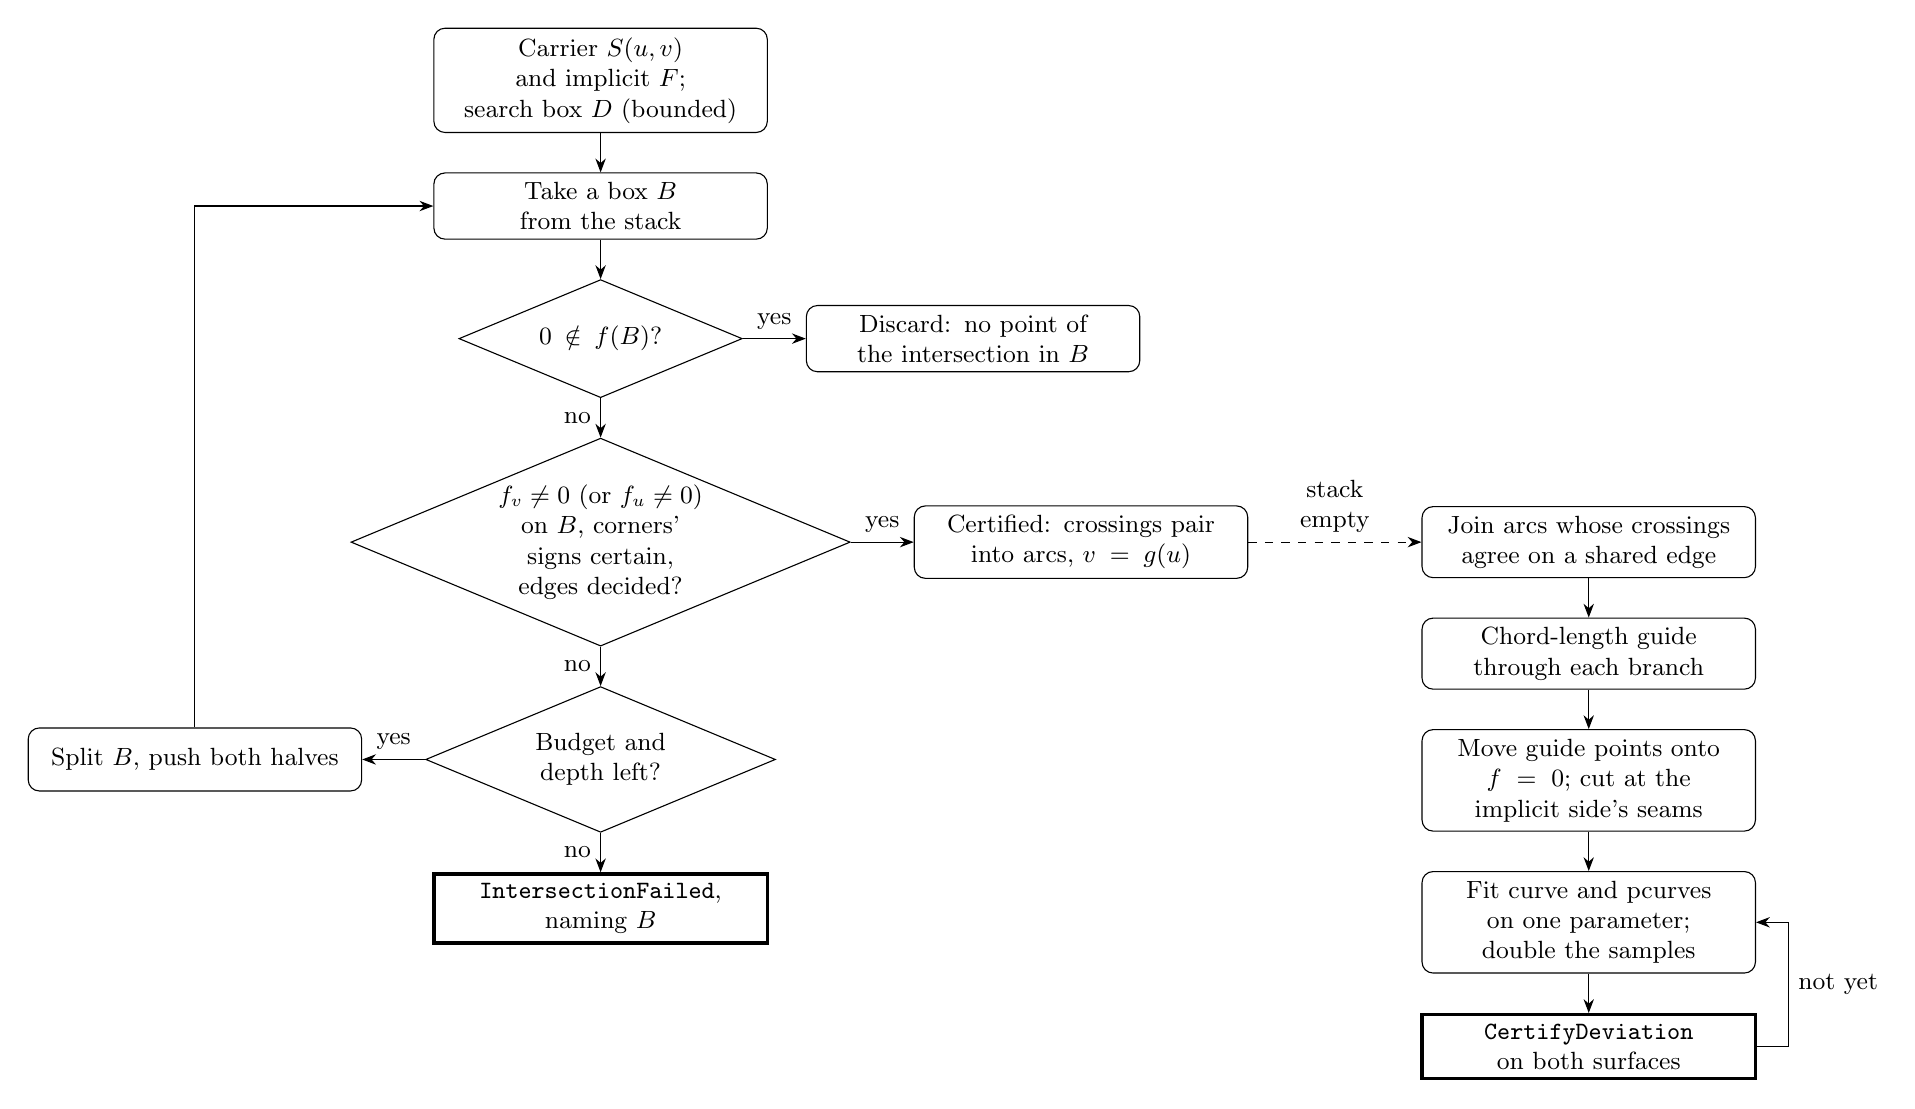
\begin{tikzpicture}[node distance=5mm and 8mm,font=\small,
    box/.style={rectangle,rounded corners,draw,align=center,text width=40mm,minimum height=8mm},
    test/.style={diamond,draw,aspect=2.4,align=center,inner sep=1pt,text width=26mm},
    stop/.style={rectangle,draw,very thick,align=center,text width=40mm,minimum height=8mm},
    ->/.style={-{Stealth[length=5pt]}}]
  \node[box] (roles) {Carrier $S(u,v)$ and implicit $F$;\\search box $D$ (bounded)};
  \node[box,below=of roles] (pop) {Take a box $B$ from the stack};
  \node[test,below=of pop] (zero) {$0 \notin f(B)$?};
  \node[box,right=of zero] (drop) {Discard: no point of the intersection in $B$};
  \node[test,below=of zero] (graph) {$f_v \neq 0$ (or $f_u \neq 0$) on $B$, corners' signs certain, edges decided?};
  \node[box,right=of graph] (arcs) {Certified: crossings pair into arcs, $v = g(u)$};
  \node[test,below=of graph] (budget) {Budget and depth left?};
  \node[box,left=of budget] (split) {Split $B$, push both halves};
  \node[stop,below=of budget] (fail) {\texttt{IntersectionFailed}, naming $B$};
  \draw[->] (roles) -- (pop);
  \draw[->] (pop) -- (zero);
  \draw[->] (zero) -- node[above] {yes} (drop);
  \draw[->] (zero) -- node[left] {no} (graph);
  \draw[->] (graph) -- node[above] {yes} (arcs);
  \draw[->] (graph) -- node[left] {no} (budget);
  \draw[->] (budget) -- node[above] {yes} (split);
  \draw[->] (split) |- (pop);
  \draw[->] (budget) -- node[left] {no} (fail);
  % After the stack empties
  \node[box,right=22mm of arcs] (join) {Join arcs whose crossings agree on a shared edge};
  \node[box,below=of join] (guide) {Chord-length guide through each branch};
  \node[box,below=of guide] (onto) {Move guide points onto $f = 0$; cut at the implicit side's seams};
  \node[box,below=of onto] (fit) {Fit curve and pcurves on one parameter; double the samples};
  \node[stop,below=of fit] (cert) {\texttt{CertifyDeviation} on both surfaces};
  \draw[->,dashed] (arcs) -- node[above,align=center] {stack\\empty} (join);
  \draw[->] (join) -- (guide);
  \draw[->] (guide) -- (onto);
  \draw[->] (onto) -- (fit);
  \draw[->] (fit) -- (cert);
  \draw[->] (cert.east) -- ++(4mm,0) |- node[pos=0.25,right,align=left] {not yet} (fit.east);
\end{tikzpicture}
\end{document}
